% !TEX TS-program = pdflatex
% !TEX encoding = UTF-8 Unicode

% This is a simple template for a LaTeX document using the "article" class.
% See "book", "report", "letter" for other types of document.

\documentclass[11pt]{article} % use larger type; default would be 10pt

\usepackage[utf8]{inputenc} % set input encoding (not needed with XeLaTeX)

%%% Examples of Article customizations
% These packages are optional, depending whether you want the features they provide.
% See the LaTeX Companion or other references for full information.

%%% PAGE DIMENSIONS
\usepackage{geometry} % to change the page dimensions
\geometry{a4paper} % or letterpaper (US) or a5paper or....
% \geometry{margin=2in} % for example, change the margins to 2 inches all round
% \geometry{landscape} % set up the page for landscape
%   read geometry.pdf for detailed page layout information

\usepackage{graphicx} % support the \includegraphics command and options
\usepackage{enumerate}


% \usepackage[parfill]{parskip} % Activate to begin paragraphs with an empty line rather than an indent

%%% PACKAGES
\usepackage{booktabs} % for much better looking tables
\usepackage{array} % for better arrays (eg matrices) in maths
\usepackage{paralist} % very flexible & customisable lists (eg. enumerate/itemize, etc.)
\usepackage{verbatim} % adds environment for commenting out blocks of text & for better verbatim
\usepackage{subfig} % make it possible to include more than one captioned figure/table in a single float
% These packages are all incorporated in the memoir class to one degree or another...

%%% HEADERS & FOOTERS
\usepackage{fancyhdr} % This should be set AFTER setting up the page geometry
\pagestyle{fancy} % options: empty , plain , fancy
\renewcommand{\headrulewidth}{0pt} % customise the layout...
\lhead{}\chead{}\rhead{}
\lfoot{}\cfoot{\thepage}\rfoot{}

%%% SECTION TITLE APPEARANCE
\usepackage{sectsty}
\allsectionsfont{\sffamily\mdseries\upshape} % (See the fntguide.pdf for font help)
% (This matches ConTeXt defaults)

%%% ToC (table of contents) APPEARANCE
\usepackage[nottoc,notlof,notlot]{tocbibind} % Put the bibliography in the ToC
\usepackage[titles,subfigure]{tocloft} % Alter the style of the Table of Contents
\renewcommand{\cftsecfont}{\rmfamily\mdseries\upshape}
\renewcommand{\cftsecpagefont}{\rmfamily\mdseries\upshape} % No bold!

%%% END Article customizations

%%% The "real" document content comes below...

\title{PoM Week 12}
\author{Martin Simon Haugaard\\cdl966}
%\date{} % Activate to display a given date or no date (if empty),
         % otherwise the current date is printed 

\begin{document}
\maketitle

\section*{12g}
\subsection{Bølgeligningen}
\subsubsection*{a}
Givet formlen:\\
$c^2 \frac{\vartheta^2}{\vartheta x^2}u(t,x) = \frac{\vartheta^2}{\vartheta t^2}u(x,t)$\\
\\
og approksimationerne\\
\\
$\frac{\vartheta^2}{\vartheta x^2} \approx \frac{u(x_{i+1}, t_j) - 2u(x_i, t_j) + u(x_{i-1}, t_j)}{h^2} $
\\
$\frac{\vartheta^2}{\vartheta t^2} \approx \frac{u(x_i, t_{j+1}) - 2u(x_i, t_j) + u(x_i, t_{j-1})}{k^2} $\\
\\
Det er muligt at se at der 5 forskellige led at operere med:
\begin{description}
\item[$U_1$:]{$u(x_{i+1}, t_j)$}
\item[$U_2$:]{$u(x_i, t_j)$}
\item[$U_3$:]{$u(x_{i-1}, t_j)$}
\item[$U_4$:]{$u(x_i, t_{j+1})$}
\item[$U_5$:]{$u(x_i, t_{j-1})$}
\end{description}
Og herudfra ser formlen således ud:\\
\\
$c^2\frac{U_1 - 2 U_2 + U_3}{h^2}=\frac{u_4 - 2 U_2 + U_5}{k^2}$\\
\\
Hvor vi ønsker at isolere $U_4$, hvilket giver følgende formel:\\
\\
$U_4 = \frac{c^2 k^2}{h^2}(U_1 - 2 U_2 + U_3) + 2 U_2 - U_5$\\
\\
Nu har vi så en formel til beregning af funktionen $u$ som funktion af $x$ til næste tidspunkt $t_{j+1}$.
\newpage

\subsubsection*{c}
Her er så resultatet af min kørsel af programmet.\\
\begin{figure}[h!]
\centering
   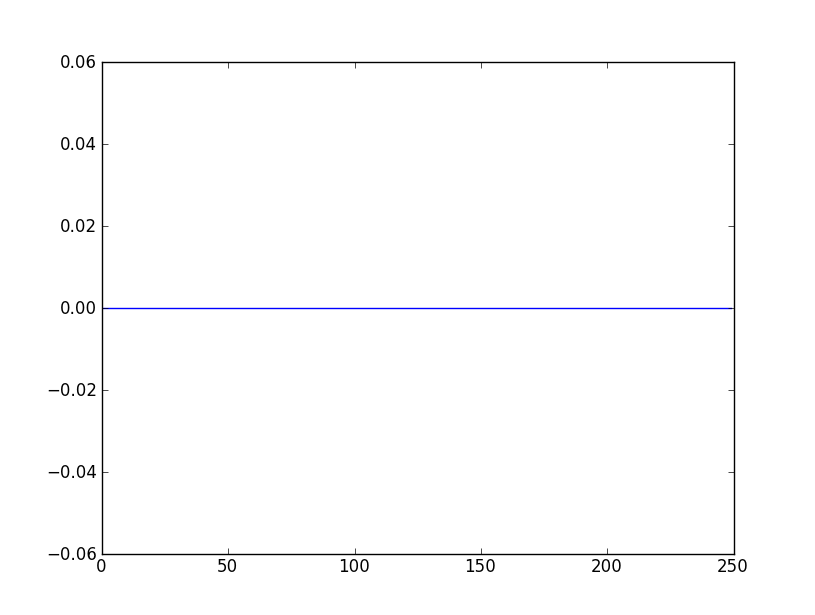
\includegraphics[width=0.5\textwidth]{bild1}
  \caption{Mit stadium uden nogen bølge i gang}
\end{figure}
\\Ovenfor ses et stadium, inden en bølge sættes i gang.
\\
\begin{figure}[h!]
\centering
   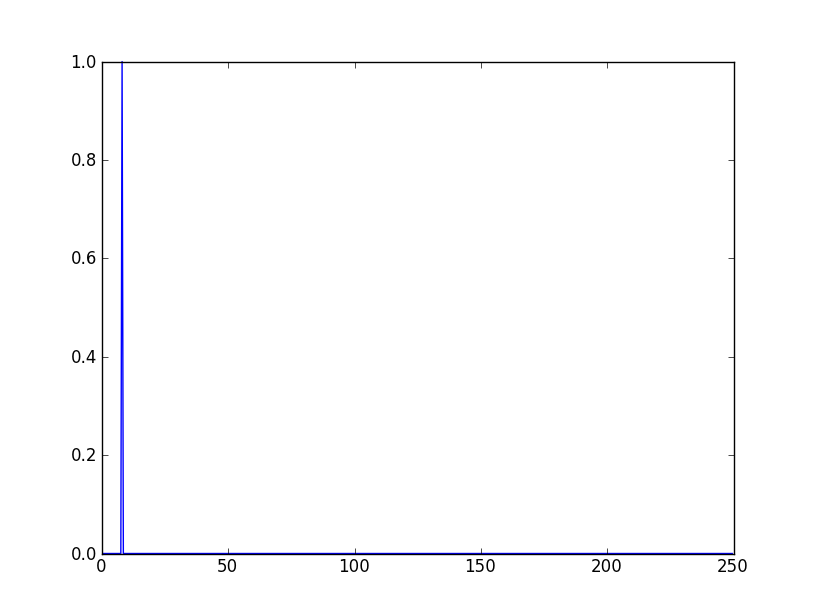
\includegraphics[width=0.5\textwidth]{bild2}
  \caption{Bølgen er startet!}
\end{figure}\\
Og der gik bølgen i gang. Den ser lidt sjov ud, da der ikke et fikspunkt som man kan sige at personen der lavet bølgen står præcist et sted. Jeg vil derfor definere bølgen som enhver x-værdi der er større eller mindre end 0.001 på min grafs y-akse.\\
\newpage
Bevæger vi os et par iterationer frem ser bølgen således ud:
\begin{figure}[h!]
\centering
   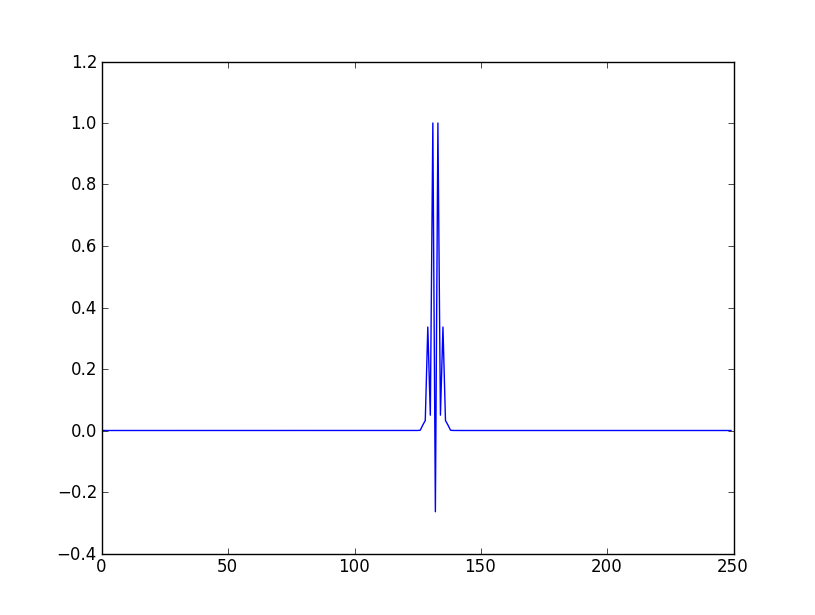
\includegraphics[width=0.5\textwidth]{midvejs}
  \caption{Bølgen er startet!}
\end{figure}
\\
Bølgen er godt halvvejs, og sådan bliver den ellers ved med at bevæge sig rundt. Når den når til kanten, fortsætter den ved x-værdi 0 og starter sådan set forfra.
\\
Det tog mig i alt 237 iterationer før min kode viste tegn på at bølgen havde nået kanten af stadium (x-værdi 250 større eller mindre end 0.001), altså en hel omgang rundt. Grunden til at det ikke tager 250 iterationer rent, er som sagt at bølgen i min model er flere felter bred.\\

\begin{figure}[h!]
\centering
   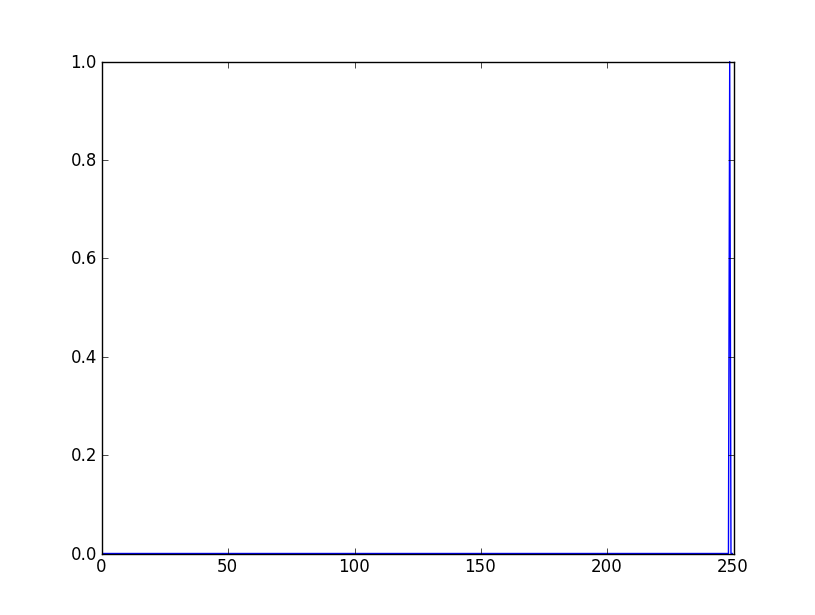
\includegraphics[width=0.5\textwidth]{slut}
  \caption{Bølgen har nået kanten af stadium, og vil begynde at wrappe rundt til starten.}
\end{figure}
Som en sjov lille bonus har jeg valgt at animere min bølge, og den kan ses ved at køre min kode (haugaard.martin.48.py) efter at alle de i rapporten viste plot er blevet lukket.\\
Koden består af 250 frames, og det viser sig at det faktisk giver en nogenlunde smooth overgang når bølgen wrapper rundt.\\
Vælger jeg at ændre på enten H eller K værdien i min kode, får jeg nogle besynderlige resultater, og jeg kan ikke påstå at det der bliver plottet er en bølge, og alle værdier bortset fra 1 og 1 resulterer i at alle tilskuere rejser sig, og i nogle tilfælde helt forsvinder i mine plots (værdierne kan ikke plottes som en graf).
\end{document}
